\section{Proposed Technique}
FIXME

\subsection{Simplicial  Complexes}
A \emph{simplicial complex} is a collection of finite sets closed under taking subsets. We refer to a set in a simplicial complex as a \emph{simplex} of \emph{dimension $p$} if it has cardinality $p+1$. Such a $p$-simplex has $p+1$ \emph{faces} of dimension $p-1$, namely the sets omitting one element, which we will denote as $[v_0,\dotsc,\hat{v}_i,\dotsc, v_p]$ when omitting the $i$'th element. While this definition is entirely combinatorial, we will soon see that there is a geometric interpretation, and it will make sense to refer to and think of $0$-simplices as \emph{vertices}, $1$-simplices as \emph{edges}, $2$-simplices as \emph{triangles}, $3$-simplices as \emph{tetrahedra}, and so forth (see Figure~\ref{fig:co-authoship-complex}).

Let $C_p(K)$ be the free real vector space with basis $K_p$, the set of $p$-simplices in 
a simplicial complex $K$. The elements of $C_p(K)$ are called \emph{$p$-chains}. The 
$p$-cochain (vector) space $C^p(K)$ is defined as the dual of $C_p(K)$, i.e. $C^p(K)=\{\hom(K,\RR)\}$. The basis of $C^p$ is given by the dual basis $K_p^*$. These vector spaces come equipped with \emph{coboundary maps}, namely linear maps defined by
\begin{align*}
  &\delta_p:C_p\to C_{p+1} \\
  &\delta_p(f([v_0,\dotsc,v_{p+1}])) = \sum_{i=0}^{p+1} (-1)^i f([v_0,\dotsc,\hat{v}_i,\dotsc,v_{p+1}])
\end{align*}
where $\hat{v}_i$ denotes that the $i$-th vertex has been omitted. 

\stefania{Change above with definition of cochain. Cochain in in a grid are pixels. Any diemnsion are the features of our simplices}
  
\begin{figure}[htpb]\label{fig:pipeline-data}
%\begin{table*}[!t]
\savebox{\tempbox}{% compute size of tabulat
\scriptsize{
\begin{tabular}{lll}
    \cmidrule(r){1-3}
    Papers   & Authors     & Citations  \\
    \midrule
    Paper I & A, B, C  & 100  \\
    Paper II &  A, B & 50\\ 
    Paper III & C, D & 4\\ 
    \bottomrule
  \end{tabular}
}}%
\settowidth{\tempwidth}{\usebox{\tempbox}}%
\hfil\begin{minipage}[b]{\tempwidth}%
\raisebox{-\height}{\usebox{\tempbox}}%
%\vspace{-7pt}
\captionof{table}{Data}%
\label{table:data}%
\end{minipage}%
\savebox{\tempbox}{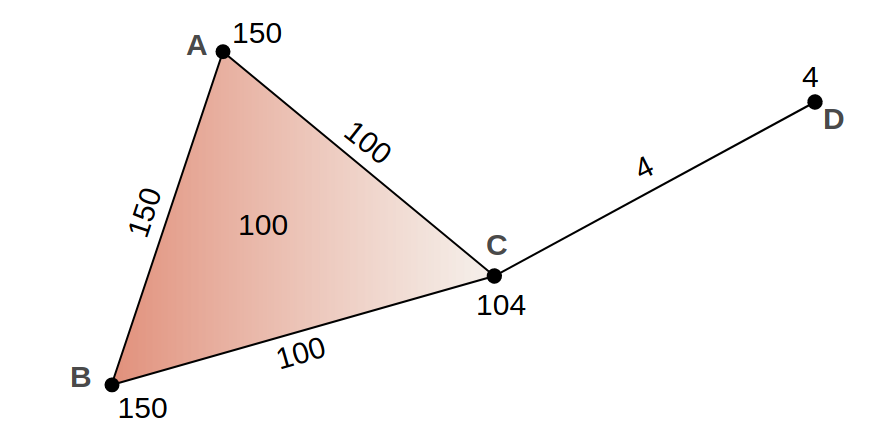
\includegraphics[height=2.3cm]{./figures/cc.png}}%
\settowidth{\tempwidth}{\usebox{\tempbox}}%
\hfil\begin{minipage}[b]{\tempwidth}%
\raisebox{-\height}{\usebox{\tempbox}}%
\captionof{figure}{Co-authorship complex}%
\label{fig:co-authoship-complex}%
\end{minipage}%
\vspace{5pt}
%\end{table*}
\caption{Example of co-authorship complex build from data}
\end{figure}

\subsection{Combinatorial Laplacians}
We are in this paper concerned with finite simplicial complexes, and assume that they are built in a way that encodes useful information about the data being studied. In particular, it is not necessary for it to come equipped with some embedding into Euclidean space, nor do we demand that it triangulates a Riemannian manifold. Therefore dualities like the Hodge star, which is used to construct the Hodge--de Rham Laplacian in the smooth setting~\cite{madsen1997calculus} that motivates us, are unavailable for our method. The same is true for discrete versions of the Hodge star, such as that of Hirani~\cite{hirani2003thesis}. To define a discrete version of the Laplacian for simplicial complexes, we simply take the linear adjoint of the coboundary operator with respect to the inner product, defining $\delta_i^\ast:C^{i+1}\to C_i$ by
\begin{align*}
  \ip{\delta_i f_1}{f_2}_{i+1} =\ip{f_1}{\delta_i^\ast f_2}_{i} \quad \forall f_1\in C^{i}(K), f_2 \in C^{i+1}(K).
\end{align*}
In analogy with Hodge--de Rham theory, we then define the \emph{degree-$i$ simplicial Laplacian} of a simplicial complex $K$ as the linear operator $\lap_i:C^i(K)\to C_i(K)$ such that
\begin{align*}
  &\lap_i = \lapu_i + \lapd_i\\
  &\lapu_i =  \delta_{i}^\ast\circ\delta_{i} : C^i(K)\to C^i(K) \\
  &\lapd_i = \delta_{i-1}\circ\delta_{i-1}^\ast : C^i(K)\to C^i(K).
\end{align*}
\stefania{Write with co-boundary}
In case $i=0$, $\mathcal{L}_0$ corresponds to the classical graph Laplacian. Observe that there are $p$ Laplacians for a complex of dimension $p$. In most practical applications, the matrices for the Laplacians are very sparse and can easily be computed as a product of sparse boundary matrices and their transposes.

\stefania{Laplacian encodes important topological information (just add references)}
\stefania{Laplacian can be seen as a message passing function on the simplices}

Our contribution is a notion of convolution for simplicial complexes using the Laplacian.


\subsection{Simplicial Neural Networks}
\begin{itemize}
\item Goal: building a convolutional NN whose input is an arbitrary $p$-cochain on a fixed simplicial ocmplex $K$
\item  Definition of Fourier Transform
\item Convolutional Filters: low degree polynomials in the frequency domain
\item Implemented using Chebyshev polynomials
\item Computational cost: good the $p$-Laplacian is localized and sparse.
\item Permutation invariant
\end{itemize}

\begin{figure}[htbp]
  \centering

\includegraphics[width=3cm]{example-image-golden}
  \caption{Maybe figures SNN} \label{fig:SNN}
\end{figure}